%! TEX root = ../main.tex
% ==============================================================
% IMMUTABLE — generated automatically, do not edit this block
%
% — Provenance ───────────────────────────────────────────────────
%   script            : analysis_scratch/paddle_contamination_study.py
%   computed_in       : analysis_scratch/paddle_contamination_study.py (Part A: truncated-stable-window AFFT via np.fft.rfft; Part B: PSD_wind = mean PSD_residual(full) − mean PSD_residual(no), evaluated at paddle bin ±0.05 Hz; incoherent subtraction A_corr = √max(0, A_fw² − E[A_wind²]))
%   plot_type         : paddle_contamination
%   data_class        : DFS
%   generated_at      : 2026-04-29T09:51:04
%   findings_doc      : analysis_scratch/paddle_contamination_findings.md
%
% — Thesis context ──────────────────────────────────────────────
%   chapter           : 04
%   caption_label     : fig:ch04_paddle_contamination
%   caption_short     : 
%
% — Filters ────────────────────────────────────────────────────
%   panel             : full
%   wind              : no, full
%   amplitude [V]     : 0.1, 0.2, 0.3
%   frequency [Hz]    : 1.3, 1.6
%   probes            : 
%   run_category      : 
%   quality_flag      : ok+probe_malfunction_secondary
%   mooring           : below_90_loose
%
% — Data provenance ────────────────────────────────────────────
%   n_runs            : 79
%   in_probes_used    : 9373/170+9373/340
%   out_probes_used   : 12400/250
%   probe_configs     : march2026_better_rearranging
%   non_final_config_n: 
%   datasets        :
%     PROCESSED-20260326-ProbePos4_31_FPV_2-tett6roof-under9Mooring-height100-lowrange
%     PROCESSED-20260327-ProbePos4_31_FPV_2-tett6roof-under9Mooring30-height100-lowrange
%   run_paths       :
%     (omitted — aggregate over > threshold runs, see datasets)
%
% — Method / numerical parameters ─────────────────────────────
%   grouper           : per (freq, amp, mooring) group; per-run correction
%   collapse_panels   : False
%   fft_window_hz     : 0.1
%   extra_params      : N_periods=[20, 40, 60, 100, 'full'], fft_window_hz=0.1, band_half_hz=0.05, welch common_grid=0-12.5 Hz @ 0.05 Hz, datasets=['20260326-ProbePos4_31_FPV_2-tett6roof-under9Mooring-height100-lowrange', '20260327-ProbePos4_31_FPV_2-tett6roof-under9Mooring30-height100-lowrange']
%
% — Summary stats cited in caption ────────────────────────────
%   stat:worst_window_drift_OUTIN : 0.0
%   stat:corr_match_median_pct : 6.84
%   stat:corr_match_max_pct : 29.79
%   stat:contamination_median_pct : 1.27
%   stat:contamination_max_pct : 2.29
%   stat:n_groups     : 12
%   stat:n_fullwind_runs : 48
%   stat:A_in_fw_over_nw_A1_median : 1.0164
%   stat:A_in_fw_over_nw_A1_max : 1.2981
%   stat:A_in_fw_over_nw_A2_median : 1.0685
%   stat:A_in_fw_over_nw_A2_max : 1.2097
%   stat:A_in_fw_over_nw_A3_median : 1.1099
%   stat:A_in_fw_over_nw_A3_max : 1.1801
%
% — Subfigures available ───────────────────────────────────────
%     FIGURES/ch04_paddle_contamination.pdf
% ── end immutable block ─────────────────────────────────────────
\begin{figure}[htbp]
  \centering
  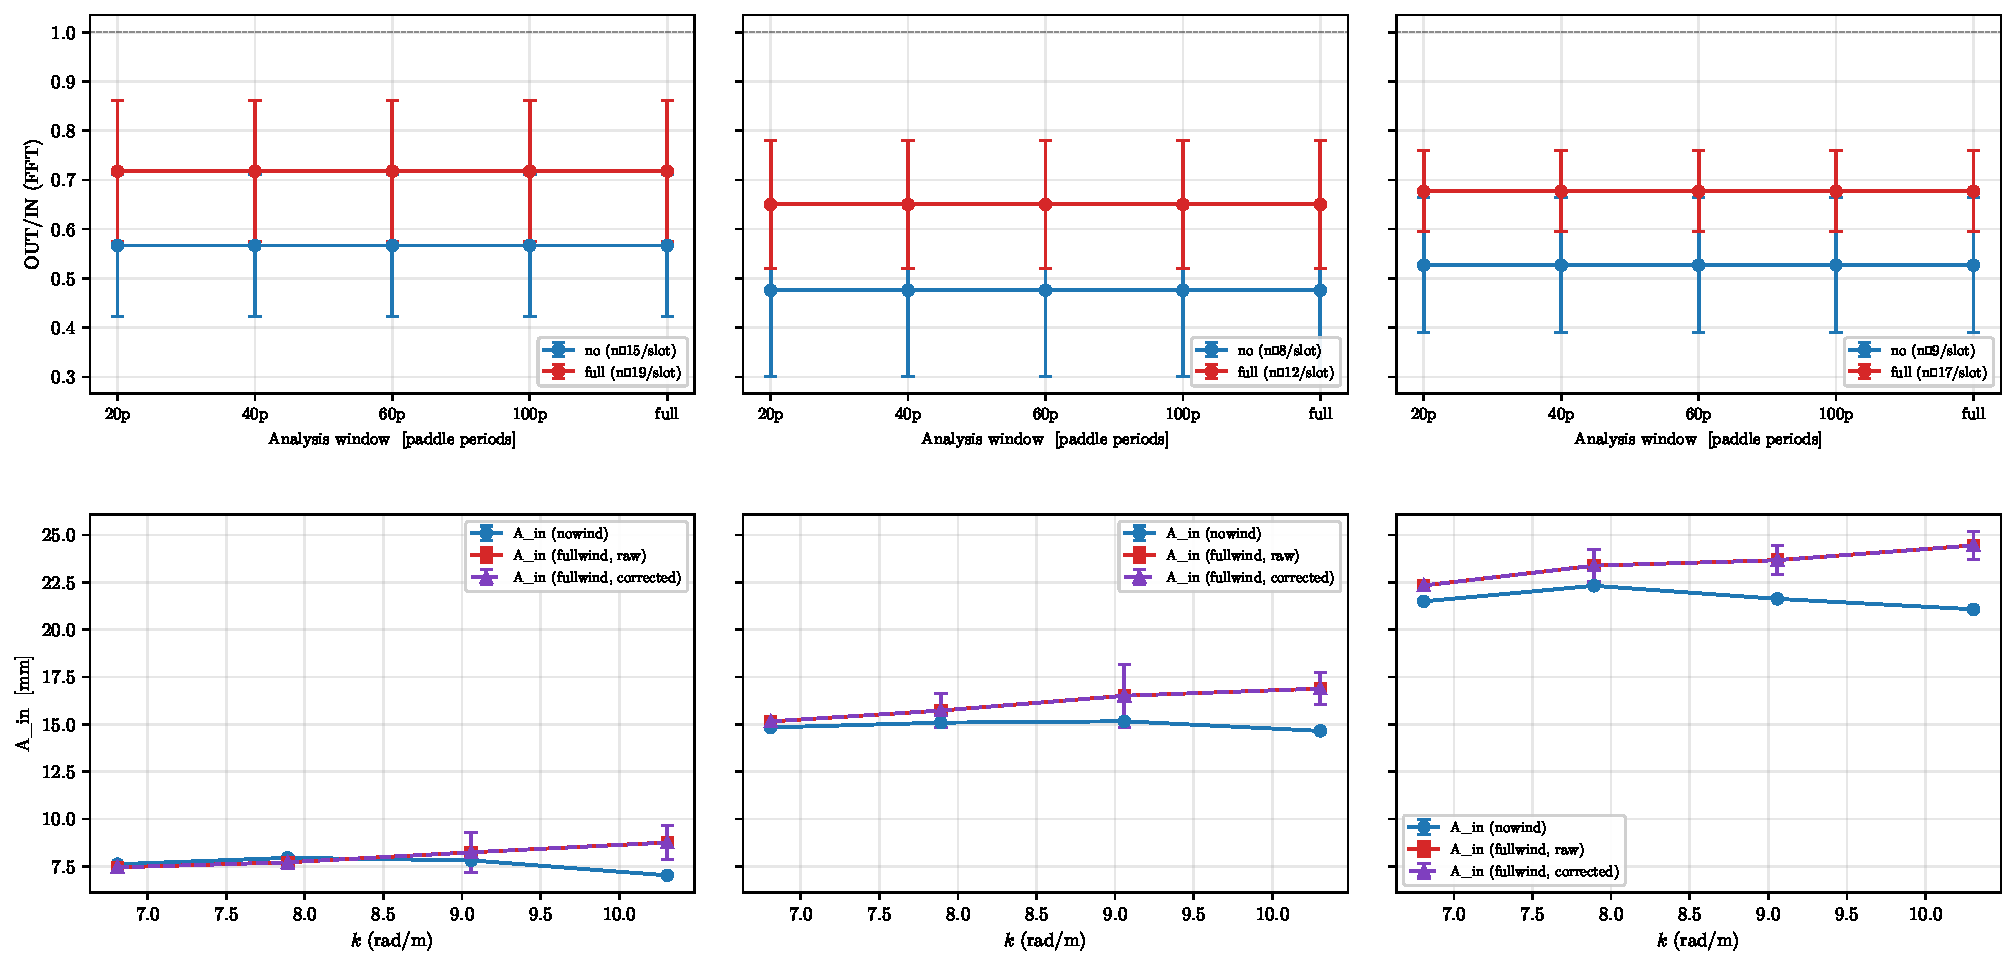
\includegraphics[width=\linewidth]{FIGURES/ch04_paddle_contamination.pdf}
  \caption{
    Top row: OUT/IN (FFT) at the paddle frequency as a function of the FFT analysis window length (20, 40, 60, 100 paddle periods and the full stable plateau), grouped by paddle drive 0.10, 0.20, 0.30\,V. Blue markers: no wind; red markers: full wind. Error bars: run-to-run standard deviation within each (amplitude, wind, window) cell. Bottom row: IN-probe amplitude at the paddle frequency versus $k$ (rad/m), one panel per amplitude. Three curves per panel: A$_{\text{in}}$ measured under no wind (blue, circles), under full wind (red, squares), and under full wind after incoherent subtraction of the wind-PSD contribution at the paddle bin (green dashed, triangles). Wind-PSD estimate per (frequency, amplitude, mooring) group: $\mathrm{PSD}_{\text{wind}}(f) = \langle\mathrm{PSD}_{\text{res}}\rangle_{\text{full}} - \langle\mathrm{PSD}_{\text{res}}\rangle_{\text{no}}$, integrated over $f_p \pm 0.05$\,Hz.
  }
  \label{fig:ch04_paddle_contamination}
\end{figure}
